%=== APPENDIX ===
%=== APPENDIX ===

\chapter{Appendix}

\section{Appendix A: API Configuration for Integration}

This appendix provides detailed API configurations and field mappings necessary for integrating SAP S/4HANA with Salesforce. It includes endpoint specifications, sample API requests, authentication mechanisms, and field-level transformations to ensure seamless data synchronization.

\paragraph{}
\textbf{S4 HANA Configuration}

\begin{figure}[h]
    \centering
     \fbox{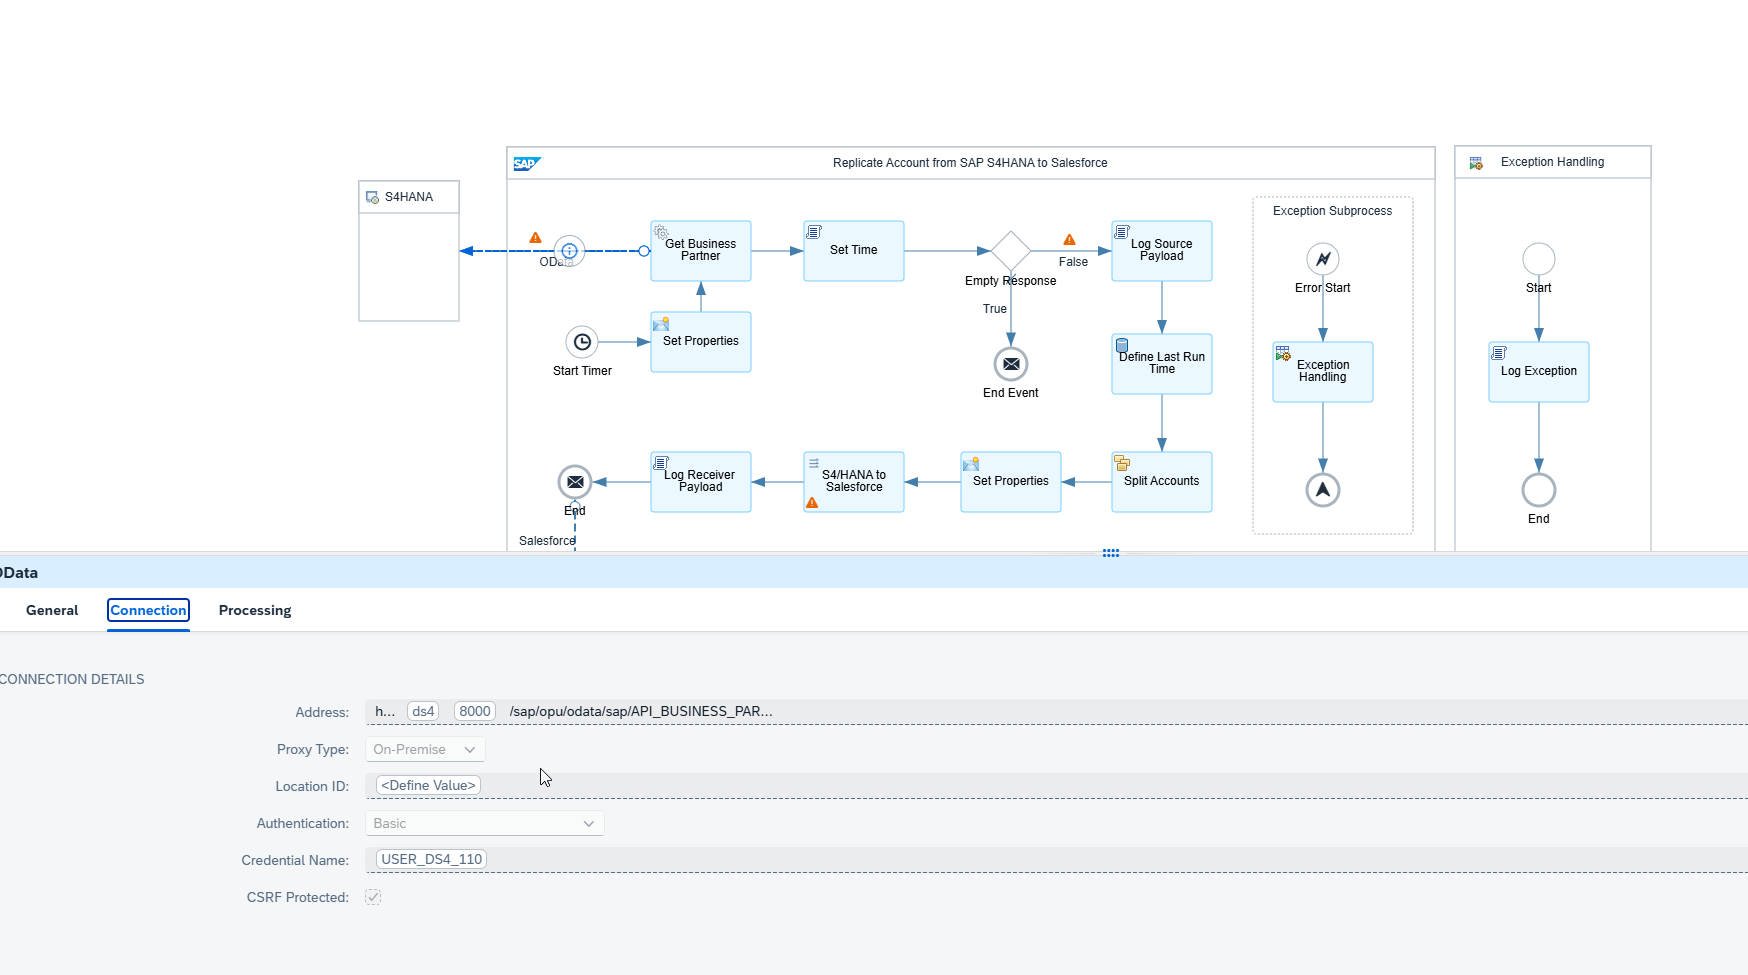
\includegraphics[width=0.95\textwidth]{Appendix/images/GetS4.png}}
    \caption{SAP S/4HANA Endpoint for Fetching Newly Created Business Partners}
    \label{fig:s4_endpoint}
\end{figure}

\noindent This image displays the \textbf{SAP BTP Integration Flow (iFlow)} used to fetch newly created Business Partners (BP) from \textbf{SAP S/4HANA} and replicate them into \textbf{Salesforce}. 

The upper section illustrates the flow's logical steps:
\begin{itemize}
    \item Fetching Business Partner data from SAP S/4HANA.
    \item Setting timestamps to track the last processed record.
    \item Handling exceptions and logging payload details.
\end{itemize}

The lower section highlights the \textbf{Connection Details} of the SAP S/4HANA endpoint:
\begin{itemize}
    \item The \textbf{OData service endpoint} (\texttt{/sap/opu/odata/sap/API\_BUSINESS\_PAR...}) used to retrieve Business Partner data.
    \item \textbf{Proxy Type}: On-Premise, indicating that the connection is routed through an \textbf{SAP Cloud Connector}.
    \item \textbf{Authentication Method}: Basic Authentication for secure access.
    \item \textbf{Credential Name}: The user credentials used to authenticate against the SAP system.
\end{itemize}

This configuration fetches only newly created Business Partners from \textbf{SAP S/4HANA} for synchronization with \textbf{Salesforce}.

\paragraph{}
\textbf{API Query Configuration}

\begin{figure}[h]
    \centering
    \fbox{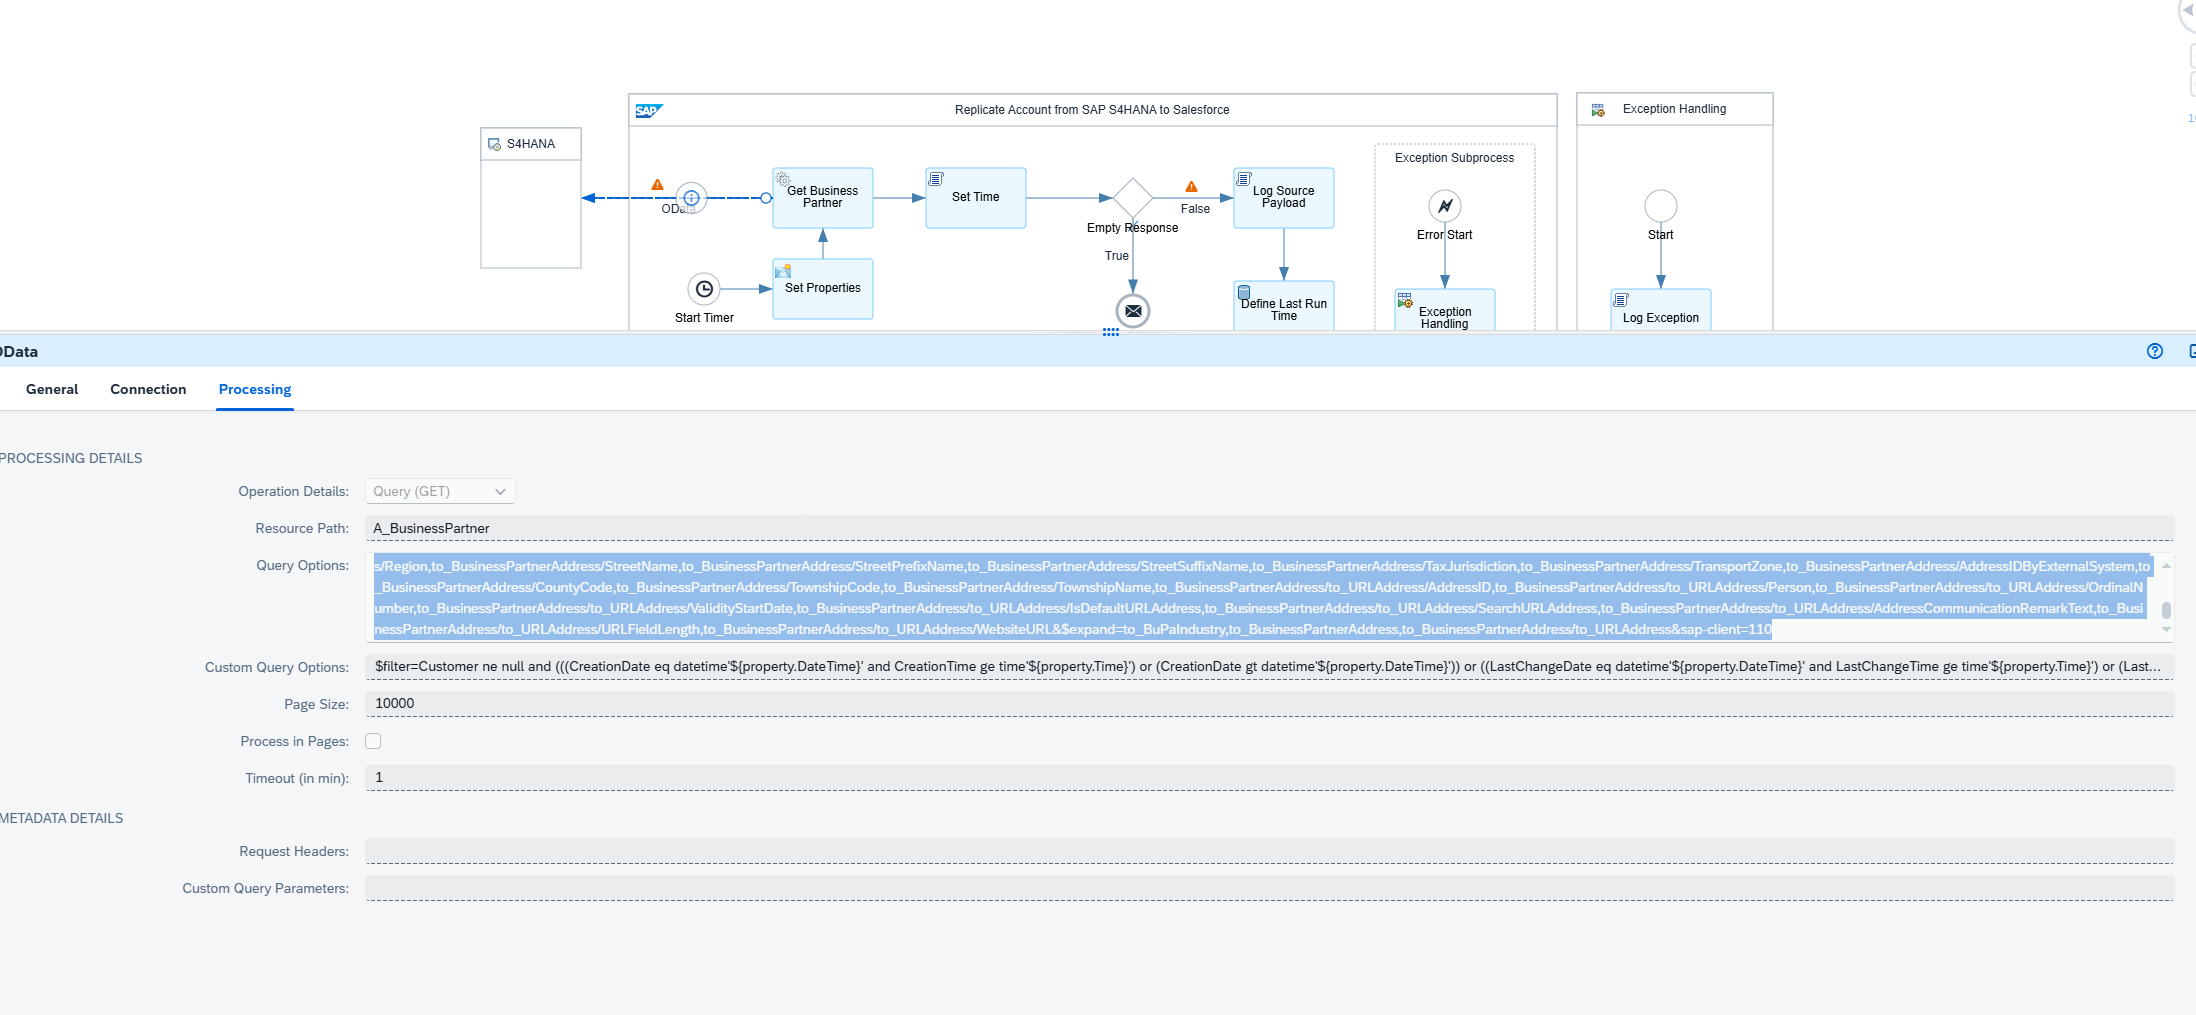
\includegraphics[width=0.95\textwidth]{Appendix/images/QueryS4.png}}
    \caption{API Query Configuration for Fetching All Business Partners in SAP S/4HANA}
    \label{fig:bp_api_query}
\end{figure}

\noindent This image displays the \textbf{SAP BTP Integration Suite's Processing Details} for the \textbf{Business Partner (BP) API query} in SAP S/4HANA. The \textbf{Query (GET) operation} is configured to retrieve \textbf{all Business Partners} using the \texttt{/A\_BusinessPartner} OData service.

Key configurations in the image include:
\begin{itemize}
    \item \textbf{Resource Path}: \texttt{/A\_BusinessPartner}, which fetches Business Partner records from SAP S/4HANA.
    \item \textbf{Query Options (\$select)}: Specifies all relevant fields, including \texttt{BusinessPartner ID}, \texttt{Name}, \texttt{Customer}, \texttt{Supplier}, \texttt{Industry}, \texttt{Address}, and other key attributes. These fields are selected to ensure that all critical information required for mapping and synchronization between SAP S/4HANA and Salesforce is retrieved. For instance, \texttt{BusinessPartner ID} serves as a unique identifier, while fields like \texttt{Name}, \texttt{Customer}, and \texttt{Supplier} provide essential business context. The inclusion of \texttt{Industry} and \texttt{Address} ensures that the integration captures comprehensive details necessary for accurate data representation in Salesforce.
    \item \textbf{Custom Query Options (\$filter)}: The condition \texttt{BusinessPartner ne null} ensures that all valid Business Partners are retrieved.
    \item \textbf{Page Size}: Set to \texttt{10,000} to optimize data retrieval in large batches.
    \item \textbf{Timeout}: Configured to \texttt{1 minute} to prevent long-running queries from failing.
\end{itemize}

This configuration ensures a \textbf{comprehensive data extraction} of all Business Partners from SAP S/4HANA, allowing seamless integration with \textbf{Salesforce} via SAP BTP.


\paragraph{}
\textbf{Salesforce Configuration}

\begin{figure}[h]
    \centering
    \fbox{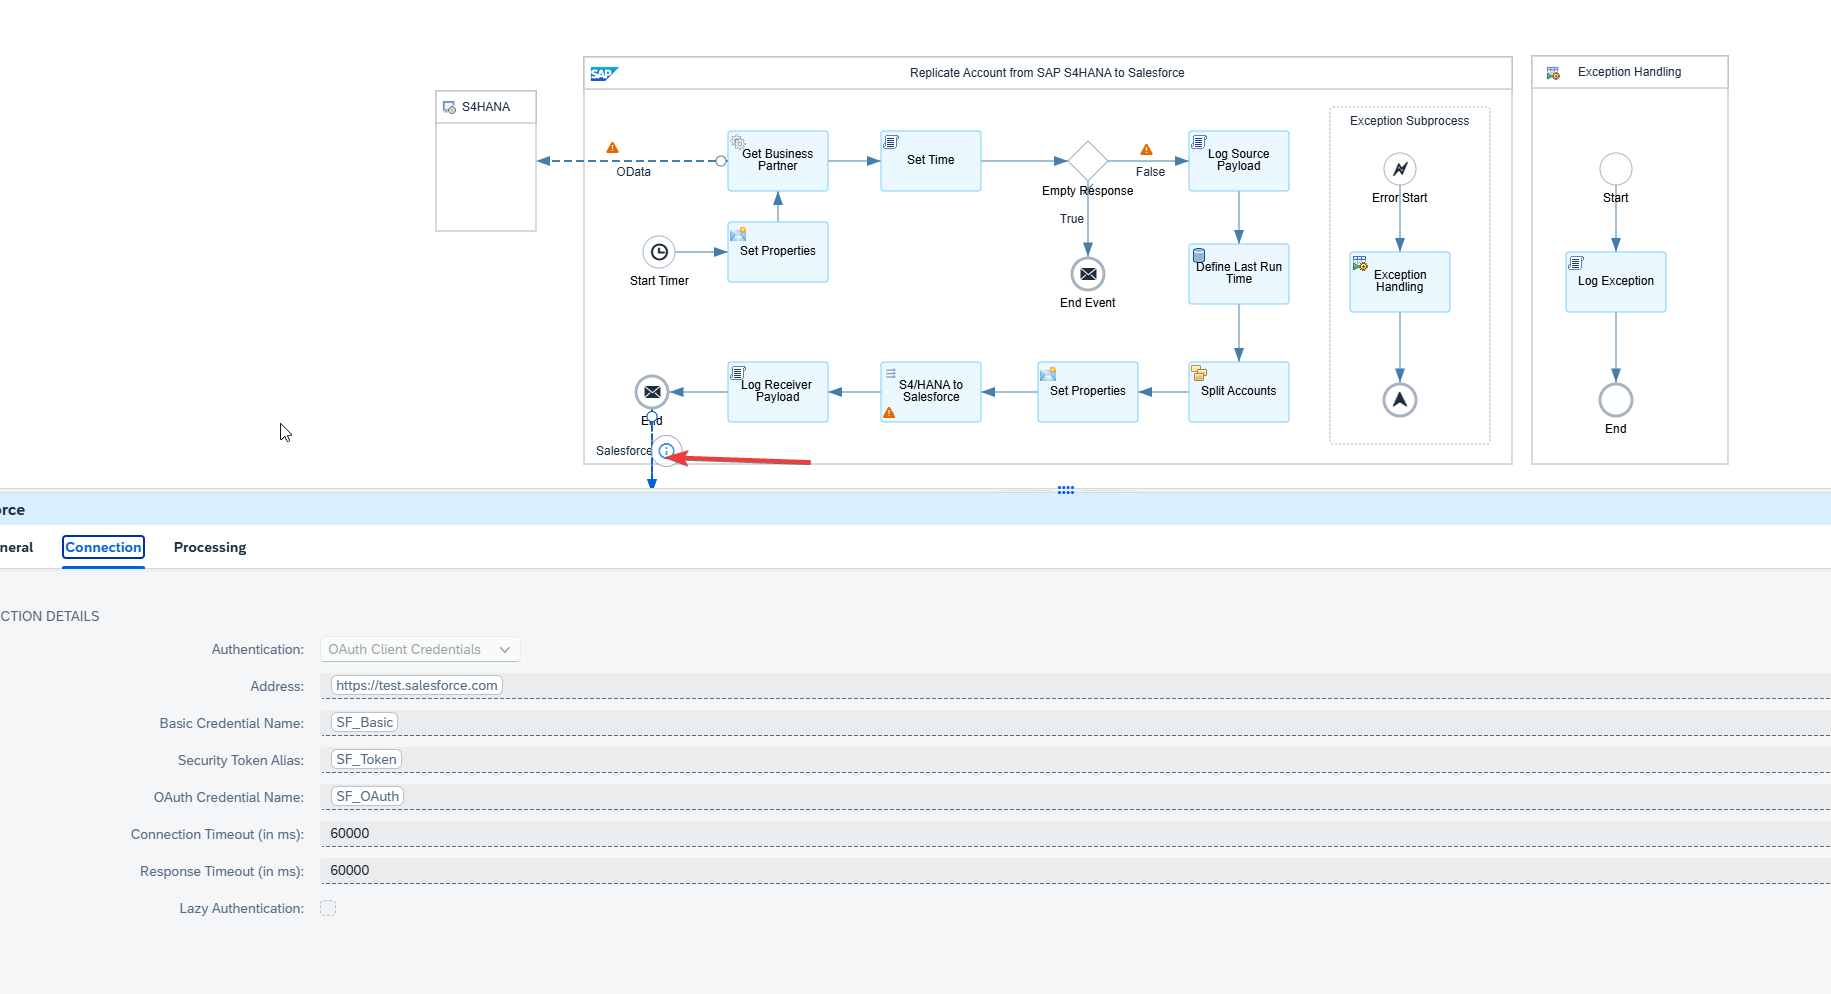
\includegraphics[width=0.95\textwidth]{Appendix/images/SF_Rec.png}}
    \caption{Salesforce Receiver API Configuration in SAP BTP}
    \label{fig:sf_receiver_api}
\end{figure}

\noindent This image displays the \textbf{Salesforce Receiver API Configuration} in the \textbf{SAP BTP Integration Suite}, which is responsible for transferring Business Partner (BP) data from \textbf{SAP S/4HANA} to \textbf{Salesforce}.

Key configurations in the image include:
\begin{itemize}
    \item \textbf{Authentication Method}: OAuth Client Credentials, ensuring secure access to the Salesforce API.
    \item \textbf{Address}: The Salesforce endpoint (\texttt{https://test.salesforce.com}) where Business Partner data is sent.
    \item \textbf{Security Token Alias}: Uses the alias \texttt{SF\_Token} for API authentication.
    \item \textbf{OAuth Credential Name}: \texttt{SF\_OAuth}, which is used for handling token-based authentication.
    \item \textbf{Connection Timeout}: Set to \texttt{60,000 ms} to allow sufficient response time from Salesforce.
    \item \textbf{Response Timeout}: Also set to \texttt{60,000 ms} to handle delays in API response processing.
\end{itemize}


\paragraph{}
\textbf{Salesforce Processing Configuration}

This configuration ensures that data synchronization between SAP S/4HANA and Salesforce is performed securely and efficiently, using OAuth-based authentication for authorization.

\begin{figure}[h]
    \centering
    \fbox{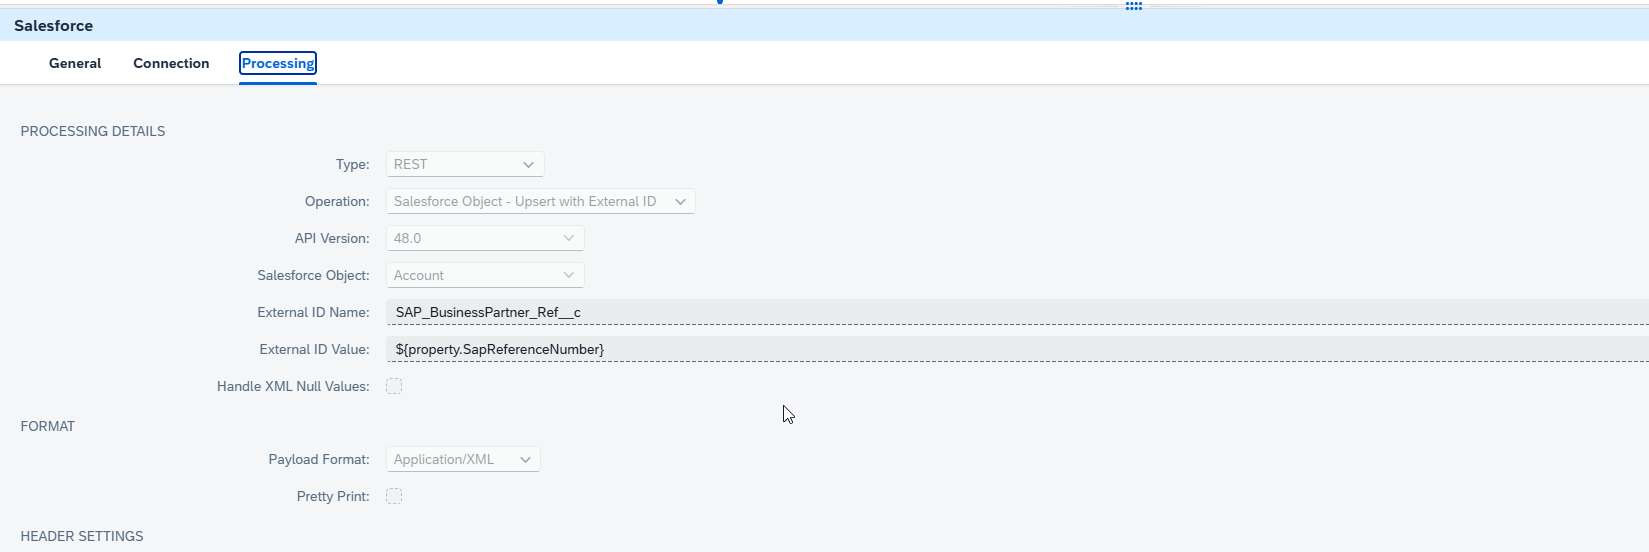
\includegraphics[width=0.95\textwidth]{Appendix/images/SF_API.png}}
    \caption{Salesforce Processing Configuration for Upserting Business Partners}
    \label{fig:sf_processing}
\end{figure}

\noindent This image displays the \textbf{Salesforce Processing Configuration} in the \textbf{SAP BTP Integration Suite}, where Business Partner (BP) data from \textbf{SAP S/4HANA} is upserted into \textbf{Salesforce}.

Key configurations in the image include:
\begin{itemize}
    \item \textbf{Type}: REST API, indicating that data is sent via a web service.
    \item \textbf{Operation}: \texttt{Salesforce Object - Upsert with External ID}, ensuring that records are either updated if they exist or created if they do not.
    \item \textbf{API Version}: \texttt{48.0}, specifying the Salesforce API version used for communication.
    \item \textbf{Salesforce Object}: \texttt{Account}, meaning the data is mapped to the Salesforce Account entity.
    \item \textbf{External ID Name}: \texttt{SAP\_BusinessPartner\_Ref\_\_c}, a custom field used to identify Business Partner records uniquely in Salesforce.
    \item \textbf{External ID Value}: \texttt{\$\{property.SapReferenceNumber\}}, dynamically passing the SAP Business Partner ID to Salesforce for matching records.
    \item \textbf{Payload Format}: \texttt{Application/XML}, specifying that data is transferred in XML format.
\end{itemize}

This configuration ensures that Business Partner records from \textbf{SAP S/4HANA} are **synchronized accurately with Salesforce**, leveraging an **upsert operation** to prevent duplicate records while maintaining data consistency.


\section{Appendix B: Video Demonstration of SAP S/4HANA and Salesforce Integration}

This appendix includes a recorded demonstration of the end-to-end integration process between SAP S/4HANA and Salesforce using SAP BTP Integration Suite. The video showcases data synchronization, API calls, and error handling in real-time.



\noindent This appendix includes video demonstrations of the SAP S/4HANA to Salesforce integration process, highlighting both a failed and a successful attempt.

\bigskip

\noindent\textbf{Failed Attempt: Account Creation to Salesforce}  

\noindent During this attempt, the integration flow encountered an error while transferring an account from SAP S/4HANA to Salesforce. The video demonstrates:
\begin{itemize}
    \item The integration flow execution in SAP BTP Integration Suite.
    \item The error message received during the process.
    \item Debugging steps taken to identify potential causes of failure.
\end{itemize}

\noindent Watch the video using the link below or by scanning the QR code:

\noindent \textbf{URL:} \href{https://drive.google.com/file/d/1qYmTXes5Tejw8vLCC0j5ul4r7GYKo6Hq/view?usp=drive_link}{\textbf{Click here to watch the failure case.}}

\begin{figure}[h]
    \centering
    
\includegraphics[width=0.3\textwidth]{Appendix/images/Fail_QR.png} % Replace with actual file name
    \caption{Scan to watch: Failed Account Creation to Salesforce}
    \label{fig:failed_video}
\end{figure}

\bigskip

\noindent\textbf{Successful Attempt: Account Creation to Salesforce}  

\noindent This video demonstrates a successful transfer of an account from SAP S/4HANA to Salesforce using the same integration flow, after resolving previous errors. It includes:
\begin{itemize}
    \item Step-by-step execution of the SAP BTP iFlow.
    \item Verification that the account is created in Salesforce without errors.
    \item Key insights into how error handling was improved.
\end{itemize}

\noindent Watch the video using the link below or by scanning the QR code:

\noindent \textbf{URL:} \href{https://drive.google.com/file/d/1YJu7LIanmCPygF6MYpwy4AShSuE6Bh88/view?usp=drive_link}{\textbf{Click here to watch the successful integration.}}

\begin{figure}[h]
    \centering
    
\includegraphics[width=0.3\textwidth]{Appendix/images/Success_QR.png} % Replace with actual file name
    \caption{Scan to watch: Successful Account Creation to Salesforce}
    \label{fig:success_video}
\end{figure}



%=== END OF CHAPTER SIX ===
\newpage
